% Chapter Template

\chapter{Turbine Derating Based on Feed Forward Signal From Upwind Turbine} % Main chapter title

\label{Chapter4} % Change X to a consecutive number; for referencing this chapter elsewhere, use \ref{ChapterX}


%----------------------------------------------------------------------------------------
%	SECTION 4-1
%----------------------------------------------------------------------------------------

\section{Introduction} \label{section4-1}

The overarching objective of this dissertation is to explore techniques for using an upwind turbine as a feed forward sensor to improve the control of downwind turbines. The previous chapter investigated a control scheme in which wind speed measurements from the upwind turbine were used to influence the blade pitch control of the downwind turbine. Initial simulations seemed promising, with the downwind turbine tracking the optimal pitch angle more closely, experiencing lower structural loading, and experiencing smaller rotor overspeeds. However, further simulations showed the control scheme was sensitive to timing errors in the feed forward data, and was likely impractical as a result. 

This chapter investigates another method for improving the control of a downwind turbine using an upwind turbine as a sensor. The control scheme investigated in this chapter has been designed to overcome the shortcomings of the control system investigated in the previous chapter while maintaining many of the same performance goals. The following sections will show that this feed forward control scheme can be very insensitive to timing errors in the feed forward data, that the control system can potentially reduce wear and tear on turbine components by reducing loads caused by large gusts of wind, and that the control system can potentially increase energy capture by reducing overspeed shutdowns in response to large gusts of wind.

The feed forward control scheme investigated in this chapter relies on selective turbine derating to reduce structural loads and rotor overspeeds. Turbine derating, sometimes referred to as turbine curtailment, is when the power produced by a turbine is intentionally reduced below the nominal operating conditions of the turbine. When a turbine is derated, the reduction in power production is generally accompanied by a reduction in structural loads as the turbine extracts less energy from the wind. There are a variety of turbine derating strategies, several of which are investigated by Deshpande and Peters \cite{deshpande2012}, but they all involve reducing either the generator speed and/or the generator torque. This is not surprising since the power generated by the turbine is approximately equal to the generator speed times the generator torque.

Turbine derating can be done for a variety of reasons, and can be done at the request of an electrical utility, or can be done by the wind plant operator in an attempt to improve plant performance. The derating requirements imposed by utilities vary, but to date, most utility requested turbine derating occurs due to lack of sufficient transmission capacity on the utility grid, or in response to high wind generation at times of low electrical load.\cite{fink2009}. A utility may also ask a wind plant to derate turbines to help utility grid frequency regulation \cite{aho2012,aho2013}. A wind plant operator may derate a turbine to reduce structural loads and increase the longevity of turbine components.\cite{biegel2013}. In applications where wind turbine maintenance is difficult to schedule, such as offshore wind farms, a turbine that experiences damage could be derated and operated at a diminished capacity until a convenient time can be found for inspection and repairs.\cite{richards2014,griffith2015}. Derating can be used to implement a "soft cut out" scheme in which the turbine will be derated in very high wind speeds instead of being completely shut down once the cut out wind speed is reached. \cite{jelavic2013} If detailed knowledge of the incoming wind speed is known, then a turbine can be dynamically derated to optimize power capture without exceeding structural loading limits.\cite{petrovic2014,petrovic2015,jelavic2013} In some cases, derating some of the turbines in a wind plant can increase the total power production of the plant.\cite{carlen2010} 
 
 The remainder of this chapter describes and investigates a control scheme that uses turbine derating in an attempt to mitigate the detrimental effects of a large wind gust propagating through a wind farm. The following section describes the derating scheme used by the feed forward controller. Section \ref{section4-3} investigates the relationship between derating, power generation, structural loads, and rotor overspeed when a turbine is subjected to a large wind gust. Section \ref{section4-4} investigates the transition between a rated and derated state. Section \ref{section4-5} describes the feed forward control system design. Section \ref{section4-6} examines the performance of the feed forward control system when subjected to a large gust of wind. 


%----------------------------------------------------------------------------------------
%	SECTION 4-2
%----------------------------------------------------------------------------------------

\section{Turbine Derating} \label{section4-2}

The power generated by a turbine is given by $P_{gen} = T_{gen}\Omega_{gen}\eta_{gen}$ where $T_{gen}$ is the generator torque, $\Omega_{gen}$ is the generator speed, and $\eta_{gen}$ is the efficiency of the generator. For a given wind speed, a turbine can be derated by reducing $\Omega_{gen}$ and/or $\eta_{gen}$ below the normal operating values. Derating a turbine typically causes a reduction in both the power generation and structural loads of the turbine. However, reducing structural loads is not always a goal of turbine derating. Therefore, the load reduction capabilities of derating are not always thoroughly examined in literature. Several derating methods have been proposed in literature. In this section three of those derating methods are investigated to determine which method is best suited for our feed forward controller.

Method 1 is based on “derating strategy C” proposed by Deshpande and Peters in "Wind turbine controller design considerations for improved wind farm level curtailment tracking."\cite{deshpande2012} In this method the rated generator speed remains unchanged and the turbine is derated by reducing the rated generator torque. The torque-speed curve of the generator torque controller is scaled to accomodate this change. Method 2 is based on the derating strategy proposed by Frost, Goebel, and Obrecht in "Integrating Structural Health Management with Contingency Control for Wind Turbines."\cite{frost2013} In this method the torque-speed curve of the torque controller remains unchanged. The turbine is derated by changing the point on the torque speed curve at which the turbine switches to a region 3 control strategy. Essentially this method derates the turbine by reducing both the rated generator torque and the rated generator speed. Method 3 is based on the derating method proposed by Petrovic and Bottasso in "Wind Turbine Envelope Riding."\cite{petrovic2015} In this method the rated generator torque remains unchanged while the turbine is derated by reducing the rated generator speed. To accommodate the reduction in the rated generator speed,the torque-speed curve of the generator torque controller is scaled and a minimum pitch angle is imposed on the blade pitch controller.


To evaluate the three derating methods, all three derating methods are simulated for a pair of test cases. In test case one the turbine has been derated by 30\% and is operating in steady 16 m/s when it experiences an extreme operating gust. In test case two the turbine has been derated by 30\% and is operating in steady 12 m/s wind when it experiences an extreme operating gust. In both test cases the extreme operating gust is defined according to IEC 61400-1 \cite{IEC2005} for a class 1 turbine in category A turbulence. Figures \ref{fig4-1} through \ref{fig4-4} illustrate how the derating strategies affect the power generation, tower base fore-aft bending moment, blade root bending moment, and rotor speed. As expected, derating the turbine by 30\% results in a 30\% reduction in power production for all three derating strategies. The deviations in power production caused by the extreme operating gust are slightly larger for derating method 3, but otherwise all three derating strategies have a very similar effect on power production. In Figure \ref{fig4-2} we see that all three derating strategies have a similar effect on tower base fore-aft bending moment before and after the extreme operating gust, with a 30\% derating corresponding to a ?????findThis???? \% reduction. However, the derating methods have differing effects on the peak tower base fore-aft bending moments induced by the extreme operating gust. Derating method 1 has a peak moment of 88.4 MNm, a 13.5\% reduction compared to a non derated turbine, while derating method 2 has a peak moment of 85.2 MNm, a 16.6\% reduction. Derating method 3 performs significantly better with a peak moment of 65.8 MNm, a 35.6\% reduction. Figure \ref{fig4-3} tells a similar story. All three derating methods have a similar effect on blade root moments when the turbine is in constant wind, but they have differing effects when the turbine is experiencing an extreme operating gust. Once again, derating method 3 out performs the other two methods with respect to reducing peak structural loads. Derating method 1 reduces the peak blade root moment by 17.5\%, method 2 reduces the  peak blade root moment by 17.0\%, and method 3 reduces the peak blade root moment by 29.5\%. Figure \ref{fig4-4} shows that the three derating strategies have very different effects on rotor speed. It is not surprising that the derating method based on reducing the rated torque (method 1) has the least effect on rotor speed, the derating method based on reducing the rated generator speed (method 3) has the greatest effect on rotor speed, and the derating method based on reducing both the rated speed and rated torque (method 2) falls somewhere in between. With derating method 1 the turbine sees a peak rotor speed of 14.18 RPM, only a 1.1\% reduction from the non-derated turbine. That peak rotor speed is 17.2\% over the turbine's rated rotor speed of 21.1 RPM. With derating method 2 the turbine sees a peak rotor speed of 13.57 RPM, a 5.4\% reduction, which corresponds to a peak overspeed of 12.1\%. With derating method 3 the turbine sees a peak rotor speed of 10.40 RPM, a 27.5\% reduction, which is not an overspeed.


\begin{figure}[htbp]
	\centering
		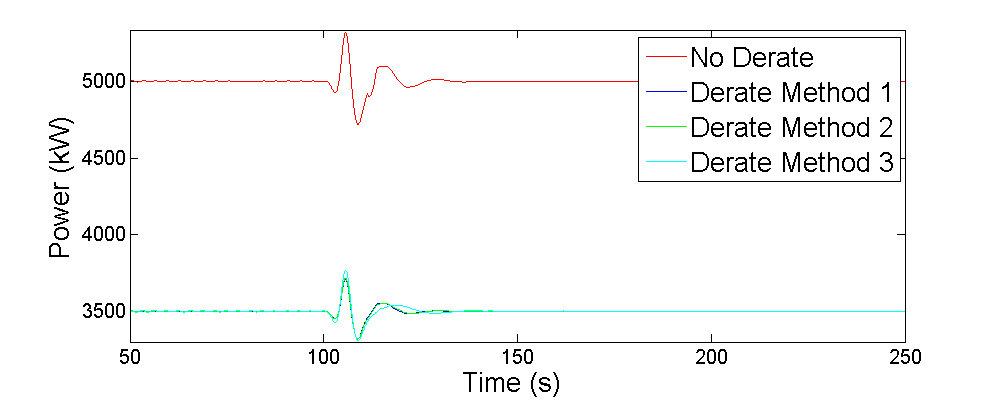
\includegraphics[width = \linewidth]{Figures/ch4Figures/fig4-1.png}
		\rule{35em}{0.5pt}
	\caption{Power generated during 16 m/s EOG for 30\% derated turbine.}
	\label{fig4-1}
\end{figure}

\begin{figure}[htbp]
	\centering
		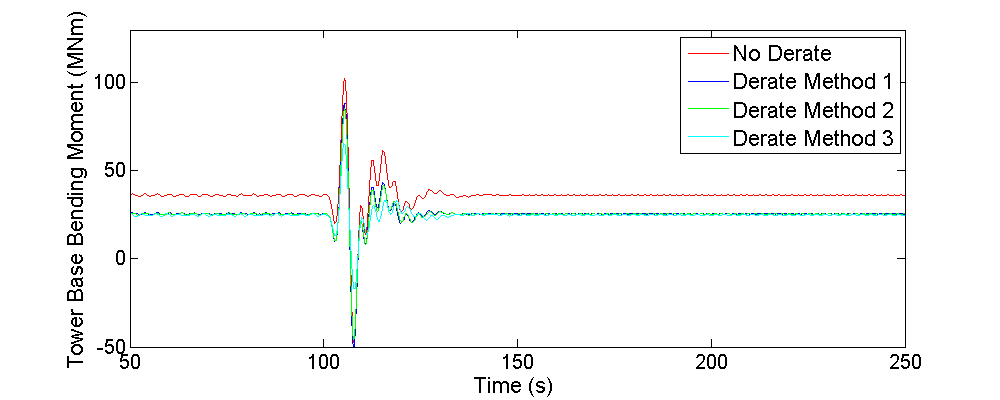
\includegraphics[width = \linewidth]{Figures/ch4Figures/fig4-2.png}
		\rule{35em}{0.5pt}
	\caption{Tower fore-aft bending moment for 30\% derated turbine during 16 m/s EOG.}
	\label{fig4-2}
\end{figure}

\begin{figure}[htbp]
	\centering
		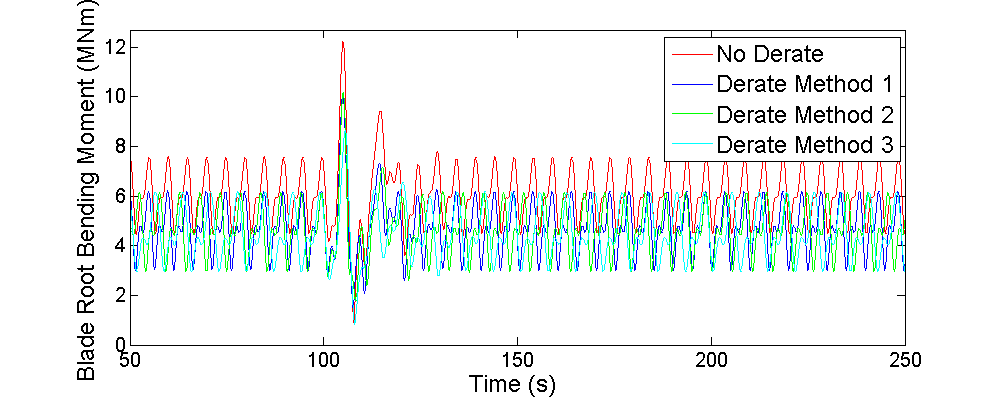
\includegraphics[width = \linewidth]{Figures/ch4Figures/fig4-3.png}
		\rule{35em}{0.5pt}
	\caption{Blade root moment for 30\% derated turbine during 16 m/s EOG.}
	\label{fig4-3}
\end{figure}

\begin{figure}[htbp]
	\centering
		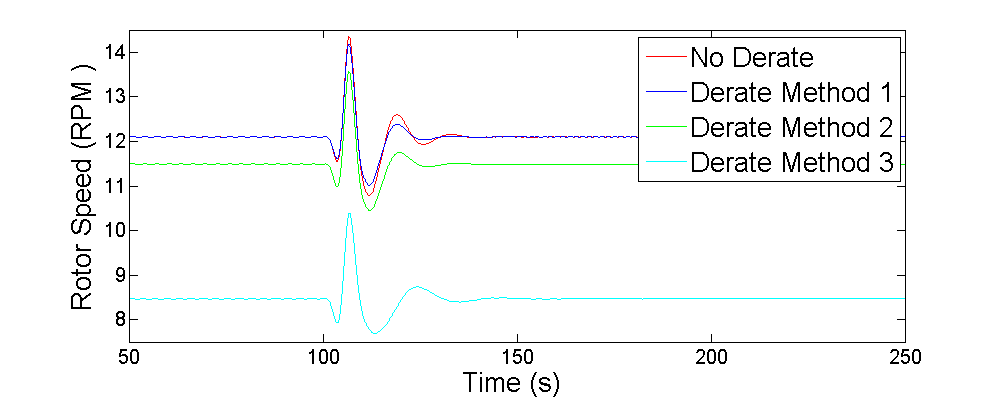
\includegraphics[width = \linewidth]{Figures/ch4Figures/fig4-4.png}
		\rule{35em}{0.5pt}
	\caption{Rotor speed for 30\% derated turbine during 16 m/s EOG.}
	\label{fig4-4}
\end{figure}


Test case 2, where a turbine is derated by 30\% and is operating in steady 12 m/s wind when it experiences an extreme operating gust, shows similar trends to test case 1. Plots of the power generation, tower base fore-aft bending moment, blade root bending moment, and rotor speed for test case two are not shown here. However, the performance observed in both test cases has been quantified and summarized in Table \ref{table4-1} and Table \ref{table4-2}. The table shows that derating method 3 is significantly better than methods 1 and 2 at reducing both the structural loads and the rotor overspeeds caused by an extreme operating gust. Since derating method 3 does the best job of mitigating the negative effects of a large gust of wind it is best suited for our feed forward controller. All further simulations described in this chapter use derating method 3. A more detailed description of derating method 3 and how it is incorporated into the NREL 5-MW controller can be found in Section \ref{section4-5}.



\begin{table}[htbp]
\centering
\label{table4-1}
\begin{tabular}{c|ccccccccc}
\hline
\hline
                                                             &                      & \multicolumn{2}{c}{\begin{tabular}[c]{@{}c@{}}Max Tower Base\\ Bending Moment\end{tabular}} &                      & \multicolumn{2}{c}{\begin{tabular}[c]{@{}c@{}}Max Blade Root\\ Bending Moment\end{tabular}} &                      & \multicolumn{2}{c}{\begin{tabular}[c]{@{}c@{}}Max Rotor\\ Speed\end{tabular}} \\ \cline{3-4} \cline{6-7} \cline{9-10} 
                                                             &                      & (MNm)                                        & Reduction                                    &                      & (MNm)                                        & Reduction                                    &                      & (RPM)                                 & Reduction                             \\ \hline
\begin{tabular}[c]{@{}c@{}}No \\ Derating\end{tabular}       &                      & 102.2                                        & -                                            &                      & 12.25                                        & -                                            &                      & 14.35                                 & -                                     \\
\\
\begin{tabular}[c]{@{}c@{}}Derating \\ Method 1\end{tabular} &                      & 88.40                                        & 13.5\%                                       &                      & 10.11                                        & 17.5\%                                       &                      & 14.18                                 & 1.1\%                                 \\
\\
\begin{tabular}[c]{@{}c@{}}Derating \\ Method 2\end{tabular} &                      & 85.19                                        & 16.6\%                                       &                      & 10.17                                        & 17.0\%                                       &                      & 13.57                                 & 5.4\%                                 \\
 \\
\begin{tabular}[c]{@{}c@{}}Derating \\ Method 3\end{tabular} &                      & 65.81                                        & 35.6\%                                       &                      & 8.64                                         & 29.5\%                                       &                      & 10.40                                 & 27.5\%  \\
\hline
\hline                             
\end{tabular}
\caption{Effect of derating methods for test case 1: 16 m/s EOG with 30\% derating.}
\end{table}


\begin{table}[htbp]
\centering
\label{table4-2}
\begin{tabular}{c|ccccccccc}
\hline
\hline
                                                             &                      & \multicolumn{2}{c}{\begin{tabular}[c]{@{}c@{}}Max Tower Base\\ Bending Moment\end{tabular}} &                      & \multicolumn{2}{c}{\begin{tabular}[c]{@{}c@{}}Max Blade Root\\ Bending Moment\end{tabular}} &                      & \multicolumn{2}{c}{\begin{tabular}[c]{@{}c@{}}Max Rotor\\ Speed\end{tabular}} \\ \cline{3-4} \cline{6-7} \cline{9-10} 
                                                             &                      & (MNm)                                        & Reduction                                    &                      & (MNm)                                        & Reduction                                    &                      & (RPM)                                 & Reduction                             \\ \hline
\begin{tabular}[c]{@{}c@{}}No \\ Derating\end{tabular}       &                      & 124.7                                        & -                                            &                      & 11.84                                        & -                                            &                      & 14.07                                 & -                                     \\
\\
\begin{tabular}[c]{@{}c@{}}Derating \\ Method 1\end{tabular} &                      & 91.36                                        & 26.7\%                                       &                      & 11.84                                        & 26.1\%                                       &                      & 13.77                                 & 2.1\%                                 \\
 \\
\begin{tabular}[c]{@{}c@{}}Derating \\ Method 2\end{tabular} &                      & 89.71                                        & 28.1\%                                       &                      & 11.78                                        & 26.5\%                                       &                      & 13.17                                 & 6.4\%                                 \\
 \\
\begin{tabular}[c]{@{}c@{}}Derating \\ Method 3\end{tabular} &                      & 70.20                                        & 43.7\%                                       &                      & 8.30                                         & 48.2\%                                       &                      & 10.38                                 & 26.2\%  \\
\hline
\hline                             
\end{tabular}
\caption{Effect of derating methods for test case 2: 12 m/s EOG with 30\% derating.}
\end{table}



%----------------------------------------------------------------------------------------
%	SECTION 4-3
%----------------------------------------------------------------------------------------

\section{Effect of Derating on Dynamic Turbine \\
		Response} \label{section4-3}

This section investigates the relationship between derating and the dynamic turbine response. In particular we are interested in determining how derating affects the structural loading and rotor overspeed a turbine experiences when subjected to a large gust. To study these relationships a series of simulations were run subjecting a derated NREL 5-MW turbine to an extreme operating gust at a variety of mean wind speeds and a variety of derating factors. The series of simulations included mean wind speeds of 6 m/s, 8 m/s, 10 m/s, 12 m/s, 14 m/s, 16 m/s, 18 m/s, and 20 m/s, as well as derating factors of 0\%, 5\%, 10\%, 15\%, 20\%, 25\%, and 30\%. For all simulations the turbine is operating in uniform, constant wind when it experiences an extreme operating gust (as defined by IEC 61400-1 \cite{IEC2005} for a class 1 turbine in category A turbulence).

Figure \ref{fig4-5} shows the relationship between derating factor and average power production for several of the mean wind speeds simulated. As expected, there is a 1 to 1 relationship between the derating factor and the reduction in power generation. Each 1\% of derating corresponds to a 1\% decrease in power production. The other wind speeds simulated also showed this same relationship.

\begin{figure}[htbp]
	\centering
		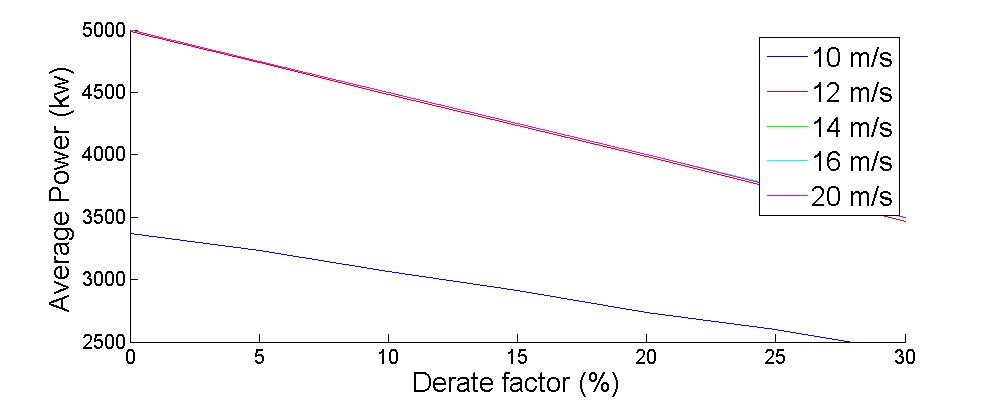
\includegraphics[width = \linewidth]{Figures/ch4Figures/fig4-5.png}
		
	\caption{Effect of derating on avg. power for EOGs at various wind speeds.}
	\label{fig4-5}
\end{figure}

Figure \ref{fig4-6} shows the relationship between derating factor and the maximum tower base fore-aft bending moment for several of the mean wind speeds simulated. One thing we see in this figure is that the turbine experiences the largest tower bending moments in simulations where the mean wind speed is equal to the rated wind speed of 12 m/s. The maximum tower bending moment decreases slowly and steadily as the mean wind speed is increased above 12 m/s. The maximum tower bending moment also decreases steadily, but more precipitously, as the mean wind speed decreases below 12 m/s. We also notice that the relationship between derating factor and maximum tower bending moment appears nearly linear. ????talk about slopes????

\begin{figure}[htbp]
	\centering
		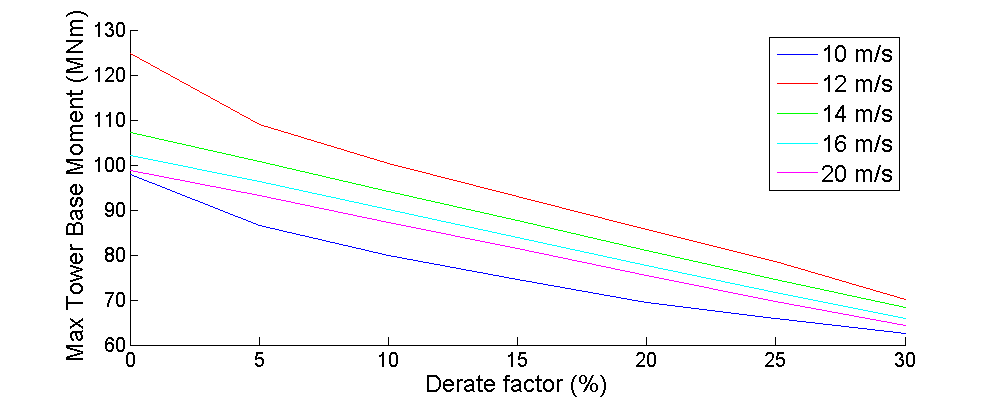
\includegraphics[width = \linewidth]{Figures/ch4Figures/fig4-6.png}
		
	\caption{Effect of derating on max tower moment for EOGs at various wind speeds.}
	\label{fig4-6}
\end{figure}

Figure \ref{fig4-7} shows the relationship between derating factor and the maximum blade root bending moment. For low derating factors we see again that highest loads occur when the mean wind speed is equal to the rated wind speed of 12 m/s and the maximum loads gradually decrease as the mean wind speed either increases or decreases away from the rated wind speed. However, at higher derating factors all of the test cases at or above the rated wind speed (12 m/s - 20 m/s) appear to converge. When the turbine is derated 25\% or 30\% the 12 m/s and 14 m/s simulations actually cause slightly larger maximum blade root moments. Again the relationship between derating factor and maximum load reduction appears nearly linear. ????talk about slopes????

\begin{figure}[htbp]
	\centering
		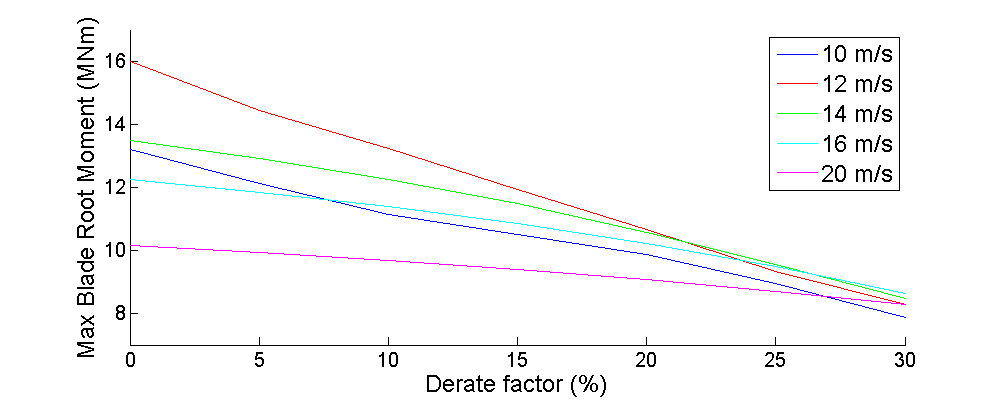
\includegraphics[width = \linewidth]{Figures/ch4Figures/fig4-7.png}
		
	\caption{Effect of derating on max blade root moment for EOGs at various wind speeds.}
	\label{fig4-7}
\end{figure}

Figure \ref{fig4-8} shows the relationship between derating factor and the maximum rotor speed, while Figure \ref{fig4-9} shows the corresponding maximum rotor overspeed. We see in these figures that the simulations with higher mean wind speeds have higher maximum rotor speeds and therefore higher maximum rotor overspeeds. As with the previous plots in this section we see a nearly linear relationship between ????not totally sure what to say here?????

\begin{figure}[htbp]
	\centering
		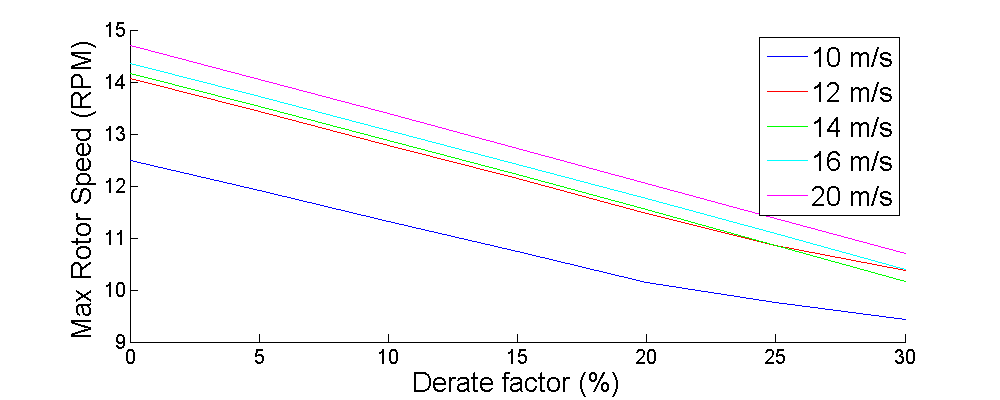
\includegraphics[width = \linewidth]{Figures/ch4Figures/fig4-8.png}
		
	\caption{Effect of derating on max rotor speed for EOGs at various wind speeds.}
	\label{fig4-8}
\end{figure}

\begin{figure}[htbp]
	\centering
		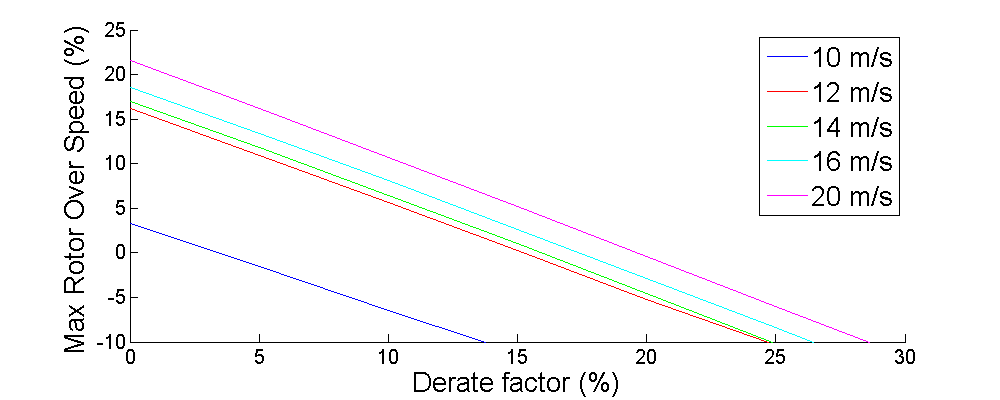
\includegraphics[width = \linewidth]{Figures/ch4Figures/fig4-9.png}
		
	\caption{Effect of derating on max rotor overspeed for EOGs at various wind speeds.}
	\label{fig4-9}
\end{figure}


%----------------------------------------------------------------------------------------
%	SECTION 4-4
%----------------------------------------------------------------------------------------

\section{Transitioning Between Rated and Derated \\
		Operation} \label{section4-4}


The previous subsection demonstrated that operating in a derated state can significantly reduce the structural loading and rotor overspeeds experienced by a turbine. However, the control scheme proposed in this chapter uses selective derating. In this control scheme the turbine will be derated when reductions in loading and rotor speed are necessary, but the turbine will operate normally when those reductions are not needed. To implement this control scheme we must understand how the turbine behaves while it is transitioning into and out of derated operation. This subsection examines the transient behavior of the turbine during these transitions and how undesirable transient behavior can be mitigated.

 When the rating of a turbine is abruptly changed the turbine exhibits undesirable transient behavior. This transient behavior is illustrated by Figures \ref{fig4-10} through \ref{fig4-12}. The figures show a test case in which the turbine operates in a steady, uniform 16 m/s wind. At t = 100 seconds the turbine is abruptly derated by 20\%, then at 200 seconds the turbine is abruptly returned to it's full rating. A 20\% derating corresponds to a rotor speed reduction from 12.1 RPM to 9.68 RPM. In Figure \ref{fig4-10} we see that when the turbine is abruptly derated the rotor undershoots the desired rotor speed by 0.94 RPM then oscillates before settling to within 2\% of the the desired rotor speed at approximately 130 seconds. When the turbine is abruptly returned to full rating it exhibits similar behavior, overshooting the desired rotor speed by 1.62 RPM (a 13.4\% overshoot) before oscillating and settling to within 2\% of the desired rotor speed at approximately 230 seconds. 

\begin{figure}[htbp]
	\centering
		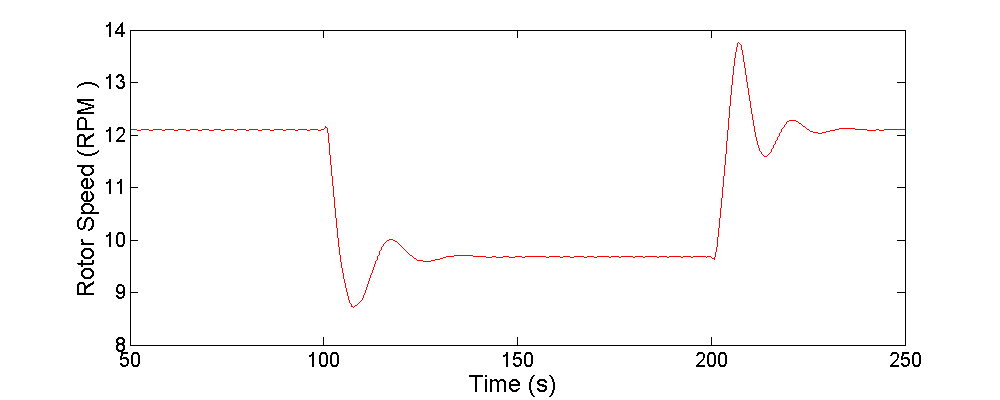
\includegraphics[width = \linewidth]{Figures/ch4Figures/fig4-10.png}
		
	\caption{Effect of sudden rating changes on rotor speed.}
	\label{fig4-10}
\end{figure}

The tower fore-aft bending moment also exhibits undesirable oscillations with settling times of approximately 30 seconds (Figure \ref{fig4-11}). These oscillations appear to have both a higher frequency component and a lower frequency component. The higher frequency oscillation (2 rad/s) corresponds to the first natural frequency of the tower. The lower frequency oscillation is caused by oscillations in the collective blade pitch. When the turbine's collective pitch controller reduces the blade pitch, in order to increase aerodynamic rotor torque and increase the rotor speed, it also increases the aerodynamic thrust on the rotor, which increases the fore-aft tower moment. Similarly, when the collective pitch controller increases blade pitch it reduces the fore-aft tower moment. 

\begin{figure}[htbp]
	\centering
		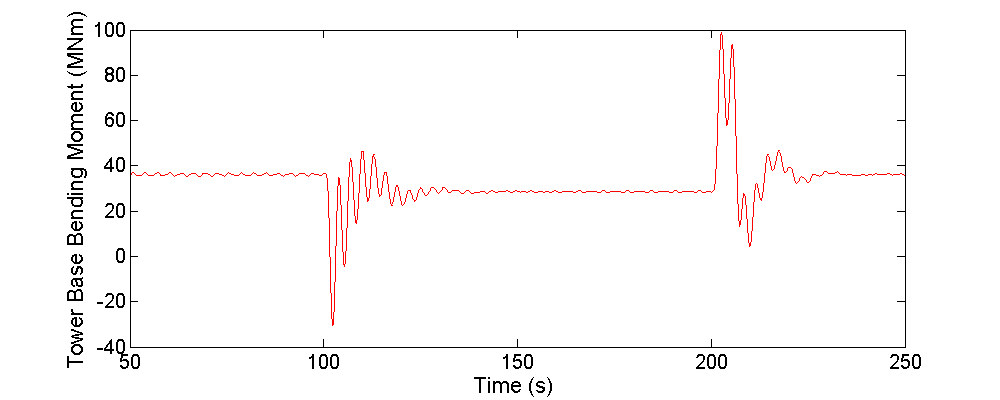
\includegraphics[width = \linewidth]{Figures/ch4Figures/fig4-11.png}
		
	\caption{Effect of sudden rating changes on tower bending moment.}
	\label{fig4-11}
\end{figure}

As Figure \ref{fig4-12} shows, the blade root bending moment also exhibits undesirable transient behavior when the turbine abruptly transitions into or out of derated operation. However, the cyclic nature of the blade root loading makes it difficult to discern the frequency or settling time of the transient behavior. Undesirable oscillations, like those shown in figures \ref{fig4-10} through \ref{fig4-12}, were seen at all wind speeds.

\begin{figure}[htbp]
	\centering
		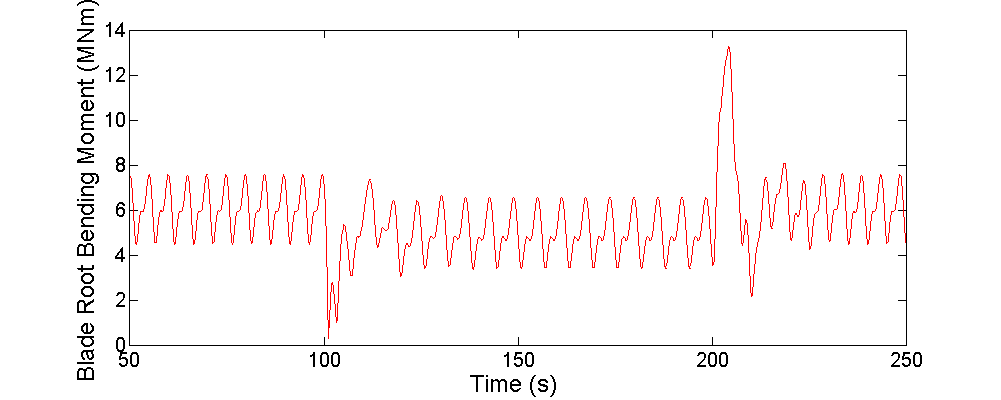
\includegraphics[width = \linewidth]{Figures/ch4Figures/fig4-12.png}
		
	\caption{Effect of sudden rating changes on blade root bending moment.}
	\label{fig4-12}
\end{figure}

We can reduce the excitation of undesirable oscillations by using a smoother transition into and out of derated operation. One way to smooth the transition is to pass derating commands through a low pass filter like the one described by the transfer function shown in Equation \ref{eq4-1}. This low pass filter is a critically damped second order system with two poles at $-P_{filter}$. Passing derate commands through this filter turns abrupt derating commands into smoother transitions, as seen in Figure \ref{fig4-13}. The 98$\%$ settling time of the filtered command is determined by the value of $P_{filter}$ and is given by $t_s = 5.8\times P_{filter}$.

\begin{equation}
	\dot{\Omega }_{Rotor}I_{Drivetrain}=T_{Aero}-T_{Gen}N_{Gear} \label{eq4-1}
\end{equation}

%\begin{figure}[htbp]
%	\centering
%		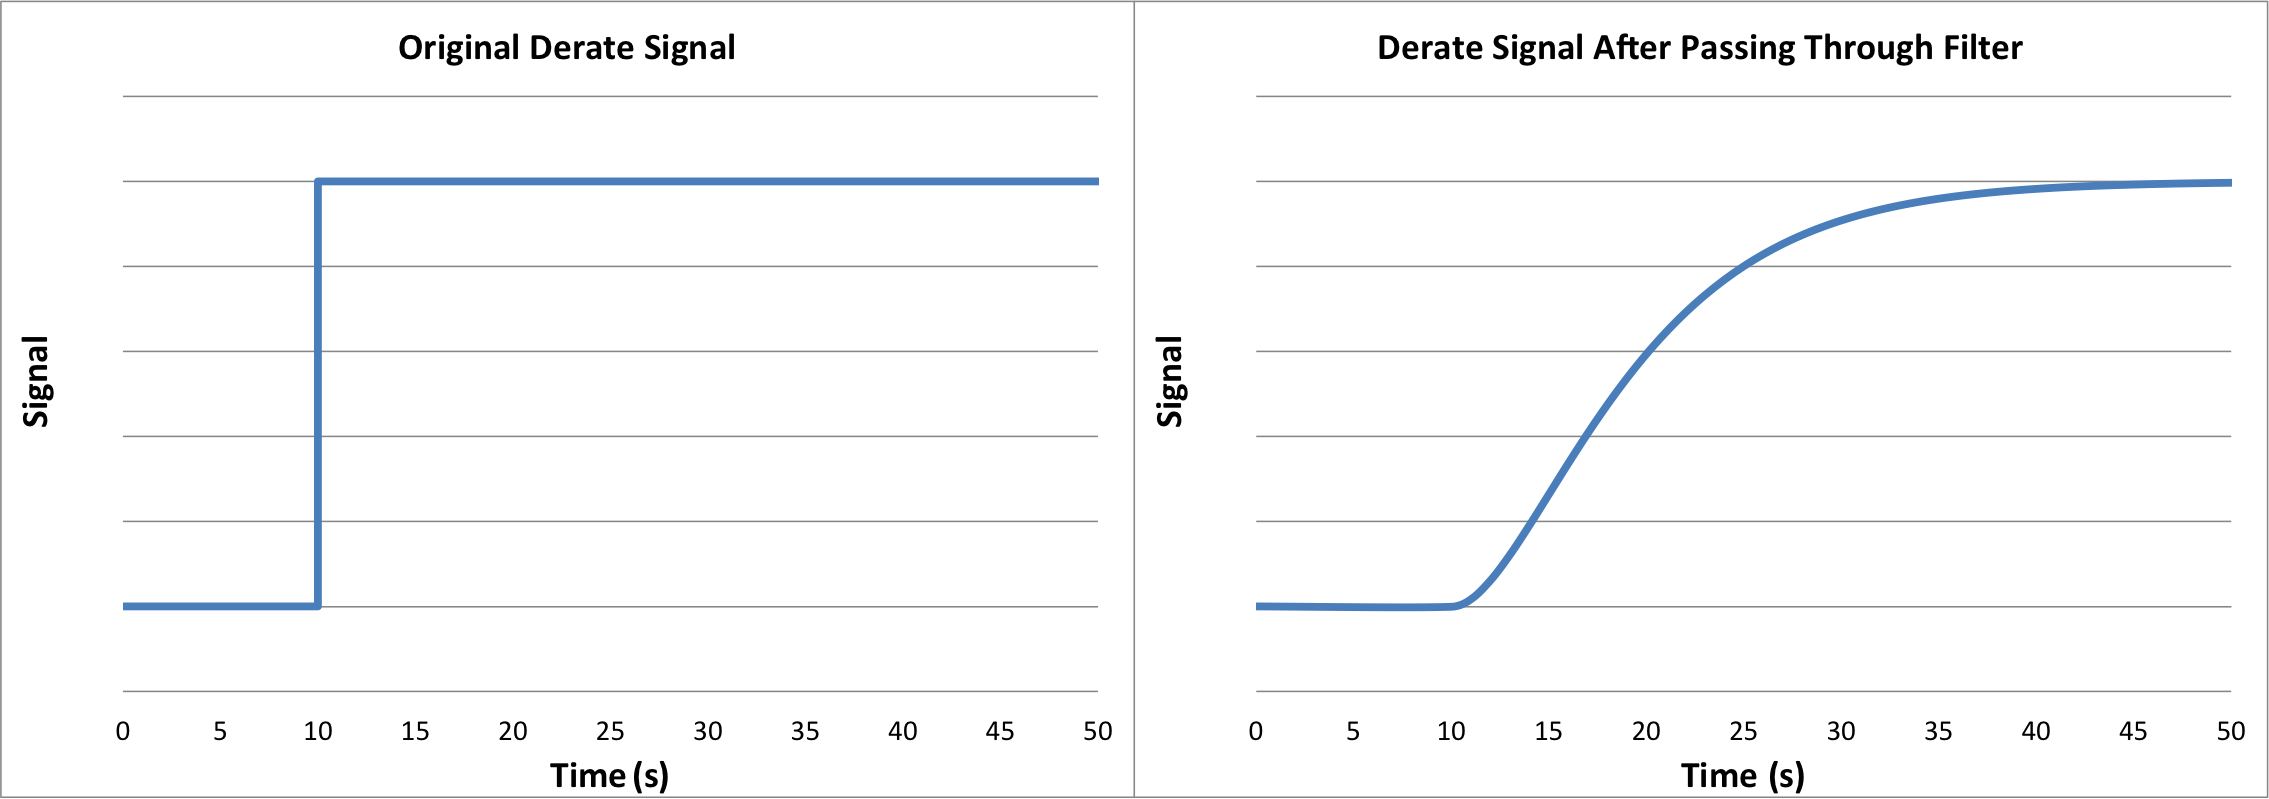
\includegraphics[width = \linewidth]{Figures/ch4Figures/fig4-13.png}
%		
%	\caption{Smoothing effect of the derating input filter.}
%	\label{fig4-13}
%\end{figure}

Choosing $P_{DRFilt}$ = 0.2 gives filtered command settling time of 29.5 seconds, which is approximately equal to the settling time of the transient oscillations caused by abrupt changes in turbine rating. As figures \ref{fig4-14} through \ref{fig4-16} show, using this filtered command to transition into and out of derated operation results in improved transient behavior while maintaining the same settling time. In Figure \ref{fig4-14} we see that the filter eliminates the oscillations, overshoots, and undershoots in rotor speed. In Figure \ref{fig4-15} we see that the filter eliminates the higher frequency oscillation. The lower frequency oscillation, caused by variations in the collective pitch angle, are still present but have reduced in magnitude. In Figure \ref{fig4-16} we see that the filter also improves transient behavior in the blade root bending moment.

\begin{figure}[htbp]
	\centering
		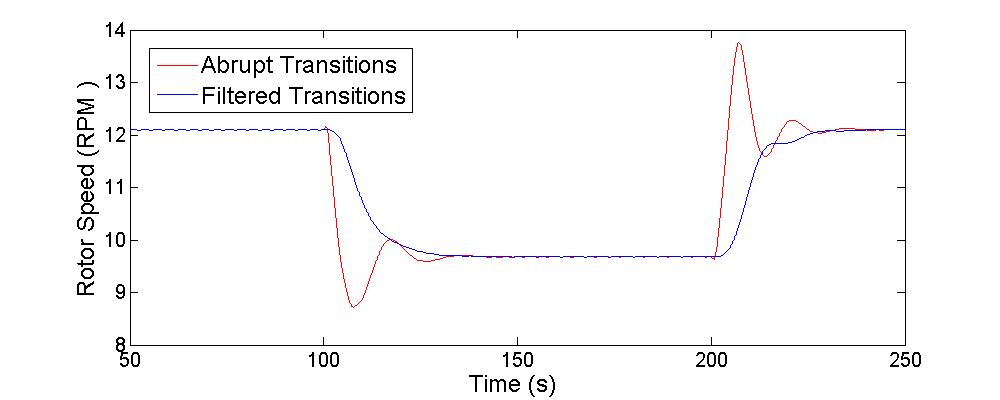
\includegraphics[width = \linewidth]{Figures/ch4Figures/fig4-14.png}
		
	\caption{Improvements in rotor behavior from filtered derate commands.}
	\label{fig4-14}
\end{figure}

\begin{figure}[htbp]
	\centering
		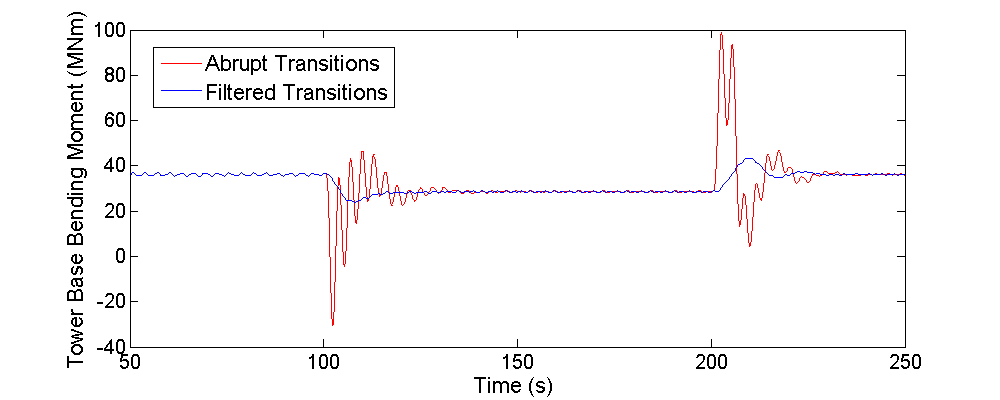
\includegraphics[width = \linewidth]{Figures/ch4Figures/fig4-15.png}
		
	\caption{Improvements in tower bending moment from filtered derate commands.}
	\label{fig4-15}
\end{figure}


\begin{figure}[htbp]
	\centering
		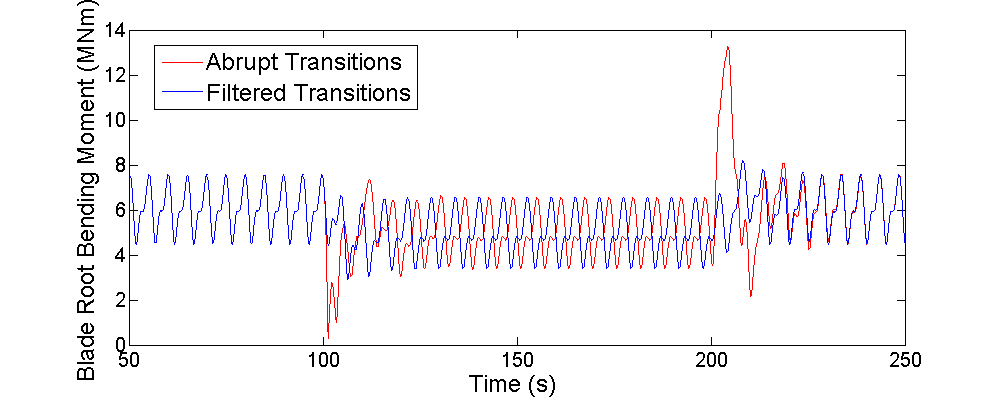
\includegraphics[width = \linewidth]{Figures/ch4Figures/fig4-16.png}
		
	\caption{Improvements in blade root moment from filtered derate commands.}
	\label{fig4-16}
\end{figure}


In general, lengthening the settling time of the filter reduces undesirable transient oscillations and reduces the magnitude of any overshoots or peak loads associated with transitioning into or out of derated operation. Figures \ref{fig4-17} through \ref{fig4-19} show the relationship between filter settling time and the maximum overshoots observed in the derating transition simulations. In practice the maximum acceptable settling time would be limited by the time it takes a gust of wind to travel from the upwind turbine to the downwind turbine. This time will depend on both the wind speed and the layout of the wind farm, however, some simple calculations can be made to help choose a reasonable filter settling time. The NREL 5-MW turbine has a rotor diameter of 126 meters. If the turbines are spaced 10 rotor diameters apart then in 12 m/s wind, the wind speed at which loads are highest and this control scheme would likely be most beneficial, a gust would travel between turbines in approximately 105 seconds. In 25 m/s wind, the highest wind speed in which the NREL 5-MW turbine will operate at all, the gust would travel between turbines in approximately 50 seconds. If the turbines are spaced 5 rotor diameters apart then a gust would travel between turbines in approximately 53 seconds for 12 m/s wind and in approximately 25 seconds for 25 m/s wind. 


\begin{figure}[htbp]
	\centering
		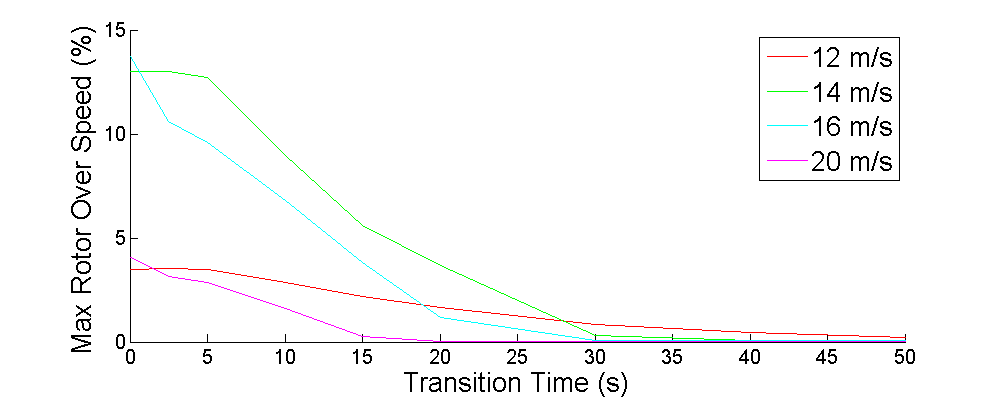
\includegraphics[width = \linewidth]{Figures/ch4Figures/fig4-17.png}
		
	\caption{Effect of input filter settling time on rotor overspeed.}
	\label{fig4-17}
\end{figure}

\begin{figure}[htbp]
	\centering
		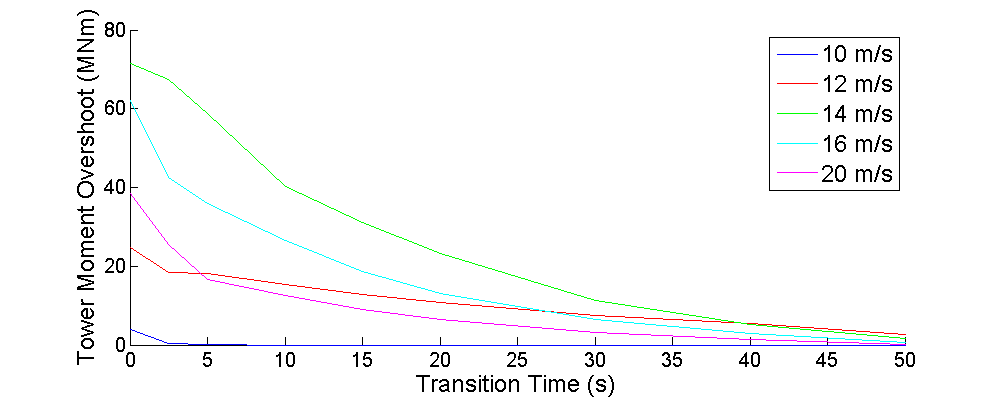
\includegraphics[width = \linewidth]{Figures/ch4Figures/fig4-18.png}
		
	\caption{Effect of input filter settling time on peak tower bending moment.}
	\label{fig4-18}
\end{figure}

\begin{figure}[htbp]
	\centering
		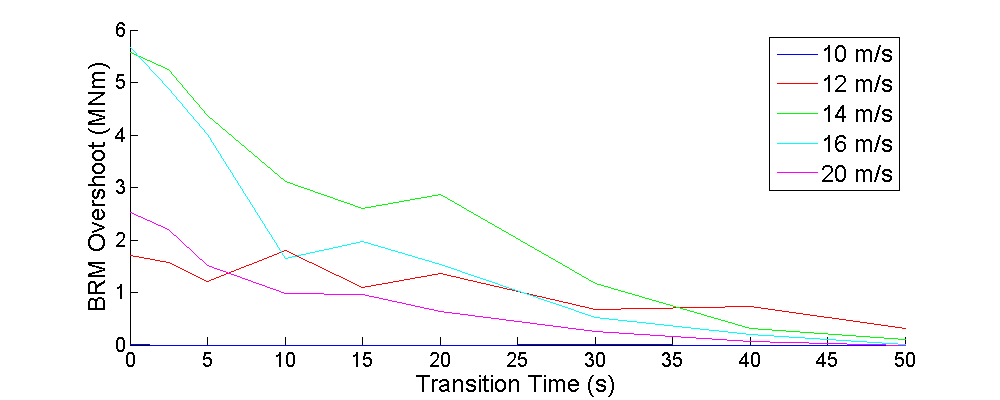
\includegraphics[width = \linewidth]{Figures/ch4Figures/fig4-19.png}
		
	\caption{Effect of input filter settling time on peak blade root moment.}
	\label{fig4-19}
\end{figure}

A low pass filter, given by equation \ref{eq4-1} with $P_{filter}$ = 0.2, will be used to smooth the turbine transitions into and out of derated operation.  $P_{filter}$ = 0.2 corresponds to a filter settling time of 29.5 seconds. Though this filter could potentially cause problems for tightly packed turbines in very high wind speeds a filter settling time of 29.5 seconds would be practical for almost all operating conditions of the NREL 5-MW turbine. As seen above, this filter also gives very good transient behavior when the turbine transitions into and out of derated operation. 

%----------------------------------------------------------------------------------------
%	SECTION 4-5
%----------------------------------------------------------------------------------------

\section{Control System Design} \label{section4-5}

As figure \ref{fig4-20} illustrates, a plant level controller will monitor the behavior of the upwind turbine and derate the downwind turbine when necessary. To determine when derating is necessary, the plant level controller will monitor the rotor speed of the upwind turbine. If the upwind turbine rotor speed exceeds some pre-defined threshold the plant level controller will interpret that as an extreme gust event and derate the downwind turbine. This threshold should be chosen based on the range of rotor speeds a turbine experiences during nominal operation, and how aggressive a plant operator chooses to be with this selective derating strategy. Therefore, in practice this threshold is likely to be site specific. 

\begin{figure}[htbp]
	\centering
		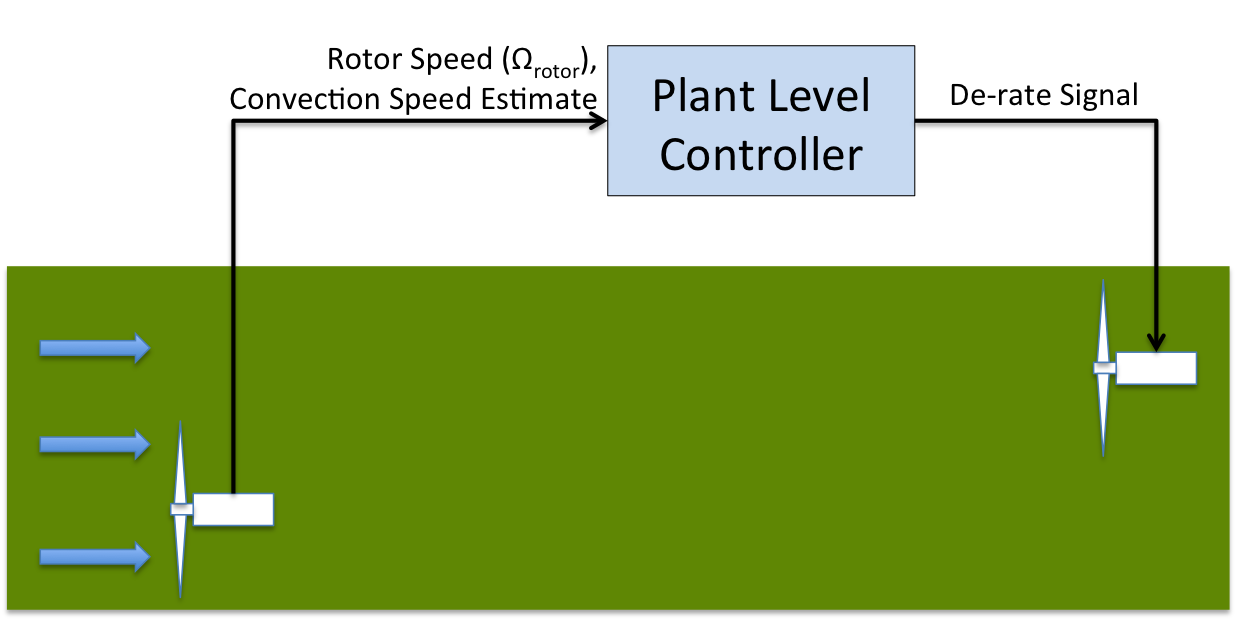
\includegraphics[width = \linewidth]{Figures/ch4Figures/fig4-20.png}
		
	\caption{Control system overview.}
	\label{fig4-20}
\end{figure}


For the simulations carried out in the following sections the threshold to initiate derating is set to 13.31 RPM (a 10\% overshoot). Section \ref{section2-2} describes a set of 66 simulations of the NREL 5-MW turbine in turbulent wind. That data set contains 7 hours of simulated turbine operation in wind speeds between 12 m/s and 22 m/s, wind speeds for which the turbine is operating in region 3 control and attempting to track the rated rotor speed of 12.1 RPM. In that 7 hours of data the rotor speed exceeds 5\% overshoot only 0.44\% of the time and never exceeds 6.76\% overshoot. A 10\% threshold to initiate derating should be sufficient to identify extreme gust events and roughly splits the difference between what the turbine sees during normal operation and a 15\% overspeed, which could potentially cause a overspeed shutdown. When derating is initiated, the downwind turbine will be derated by the maximum rotor overspeed observed in the extreme gust event minus 5\%. 

As shown in section \ref{section4-3}, derating the downwind turbine will reduce the structural loads and rotor overspeed caused by the extreme gust event. As a result the downwind turbine will experience reduced structural damage and avoid a possible overspeed shutdown when the extreme gust arrives. Once the extreme gust has passed the downwind turbine the downwind turbine will be returned to full rated operation. Several methods can be used to determine when the downwind turbine should be derated ($T_{startDerate}$) and when it is safe for the downwind turbine to return to full rated operation ($T_{endDerate}$). Two of those methods are examined in the following paragraphs.

One method of determining when to derate the downwind turbine is to use an estimate of the gust's convection speed. The time it takes for a gust of wind to travel from the upwind turbine to the downwind turbine is given by $t = D/U_{conv}$, where $D$ is the downwind distance between the turbines and the convection speed $U_{conv}$ is the rate at which wind speed fluctuations propagate downwind. Section \ref{section2-4} examined a method for estimating wind speed using blade pitch, rotor speed, generator torque, and known dynamics of the turbine. Section \ref{section2-5} examined using that wind speed estimation technique to estimate the convection speed. 

Large rotor overspeeds occur when the turbine is operating at or above the rated wind speed. For the NREL 5-MW turbine that means that large overspeeds will occur when the wind speed is between 12 and 25 m/s. Section \ref{section2-5} analyzed 7 hours of simulated turbine operation in those wind conditions. With a 60 second averaging time, the mean error in convection speed estimates was approximately 3.2\% and the largest error seen in a convection velocity estimate was approximately 5.6\%. To improve this control scheme's robustness to errors in convection velocity estimation we can base our derate timing on a larger error than was seen in those results. If the plant level controller begins and ends the derate signal based on Equations \ref{eq4-2} and \ref{eq4-3} then the control system will accommodate extreme wind events traveling up to 20\% faster or 20\% slower than the convection velocity estimate. $t_{Event}$ is the time at which the upwind turbine experiences an unacceptably large overspeed. Recall that $t_{conv}$ is the estimated time it will take for the gust of wind to travel from the upwind turbine to the downwind turbine and $t_s$ is the time required for the turbine to smoothly transition into derated operation. This system could experience problems if the upwind turbine experienced an overspeed shutdown, as convection velocity estimates would no longer be available.


\begin{equation}
	t_{DR_start} = t_{Event} + 0.8 \times t_{conv} - t_s \label{eq4-2}
\end{equation}

\begin{equation}
	t_{DR_end} = t_{Event} + 1.2 \times t_{conv} \label{eq4-3}
\end{equation}



Another method of determining when to derate the downwind turbine is to develop worst case scenarios based on the operating conditions of the turbine. For the NREL 5-MW turbine we have determined that large rotor overspeeds will occur when in wind speeds between 12 m/s and 25 m/s. If the downwind turbine is 10 rotor diameters (1260 m) behind the upwind turbine and the convection speed is somewhere between 12 and 25 m/s it would take a gust of wind between 105 and 50.4 seconds to travel from the upwind turbine to the downwind turbine. Therefore, if the turbine is derated from 50.4 seconds to 105 seconds after the upwind turbine experiences an unacceptable overspeed the downwind turbine should be in derated operation when the gust arrives no matter what the wind speed is. To add more safety margin we can base our worst case scenario on an even wider range of convection velocities. If the transition to derated operation is based on a 30 m/s convection time and the transition out of derated operation is based on an 8 m/s wind the derate signal will be based on equations \ref{eq4-4} and \ref{eq4-5}, where 42 seconds is the time required for a gust traveling 30 m/s to reach the downwind turbine and 157.5 is the time required for a gust traveling 8 m/s to reach the downwind turbine.  A similar calculation can be done for other turbines and/or other turbine to turbine spacing. Though this method derates the downwind turbine for longer than is strictly necessary it is simple, robust, and does not require an estimate of the convection velocity.

\begin{equation}
	t_{DR_start} = t_{Event} + 42 seconds - t_s \label{eq4-4}
\end{equation}

\begin{equation}
	t_{DR_end} = t_{Event} + 157.5 seconds \label{eq4-5}
\end{equation}






**Maybe explain how derating signal is processed.?????**


%----------------------------------------------------------------------------------------
%	SECTION 4-6
%----------------------------------------------------------------------------------------

\section{System Performance} \label{section4-6}

The following sections examine the performance of the selective derating feed forward control system. A two turbine system is simulated using FAST using the method described in Section \ref{section3-2}. The upwind turbine, with a conventional closed loop turbine controller,  is simulated first. The dynamic response of that turbine is recorded and post processed to generate feed forward control signals. This post processing simulates the plant level controller. Finally the downwind turbine, with feed forward control, is simulated. By comparing the dynamic behavior of both simulations we determine the effect of the feed forward control system.

%-----------------------------------
%	SUBSECTION 4-6-1
%-----------------------------------
\subsection{Response to IEC Extreme Operating Gust} \label{section4-6-1}

The first simulation case is a uniform wind field with an extreme operating gust (EOG). The extreme operating gust has been defined according to IEC 61400-1 \cite{IEC2005} for an NREL 5-MW turbine operating in 16 m/s wind. This is the same test case used to analyze the performance of feed forward optimal pitch control in Sections \ref{section3-4-1} and \ref{section3-5-1}, however the EOG has been shifted to occur 200 seconds after the start of the simulation, as shown in Figure \ref{fig4-22}. This shift will ensure that transient derating behavior will not overlap with any of the transient turbine start up  behavior at the beginning of the simulation.

\begin{figure}[htbp]
	\centering
		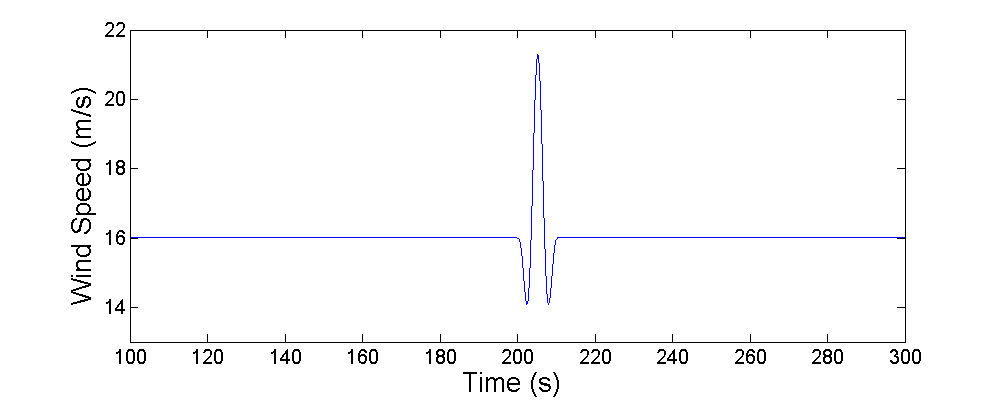
\includegraphics[width = \linewidth]{Figures/ch4Figures/fig4-22.png}
		
	\caption{Extreme operating gust.}
	\label{fig4-22}
\end{figure}

Figures \ref{fig4-23} through \ref{fig4-26} show how feed forward selective derating control affects the rotor speed, tower base fore-aft bending moment, blade root moment, and power generation of the downwind turbine. Table \ref{table4-3} quantifies and summarizes several important performance metrics. Two methods were used to time the derating of the downwind turbine. As discussed in Section \ref{section4-5}, the first method uses an estimate of the gust confection speed to determine when to derate the turbine. The second, more conservative,  method derates the downwind turbine over a longer period of time, but does not require an estimate of the convection speed. Both methods have an identical effect on rotor speed and peak structural loads, but they affect power generation differently. 

Figure \ref{fig4-23} shows that the upwind turbine experiences an 18.76 \% rotor overspeed due to the EOG, potentially enough to cause an emergency shutdown of the turbine, but the feed forward controller reduces the rotor overspeed in the downwind turbine to 4.96\%. In Figures \ref{fig4-24} and \ref{fig4-25} we see that both the upwind and downwind turbines experience large structural loads due to the EOG, but the loads experienced by the downwind turbine are smaller. The feed forward controller has reduced the maximum tower base fore-aft bending moment by 21.9\% and the maximum blade root bending moment by 14.7\%. 

\begin{figure}[htbp]
	\centering
		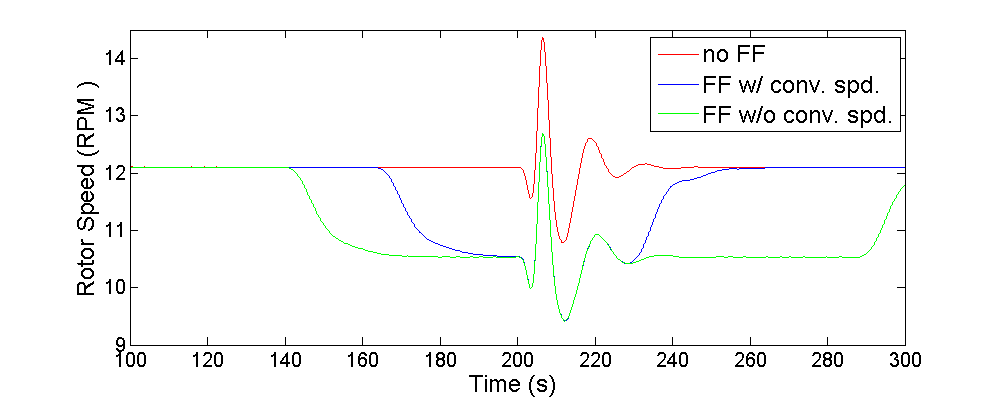
\includegraphics[width = \linewidth]{Figures/ch4Figures/fig4-23.png}
		
	\caption{Rotor speed for turbine subjected to extreme operating gust.}
	\label{fig4-23}
\end{figure}

\begin{figure}[htbp]
	\centering
		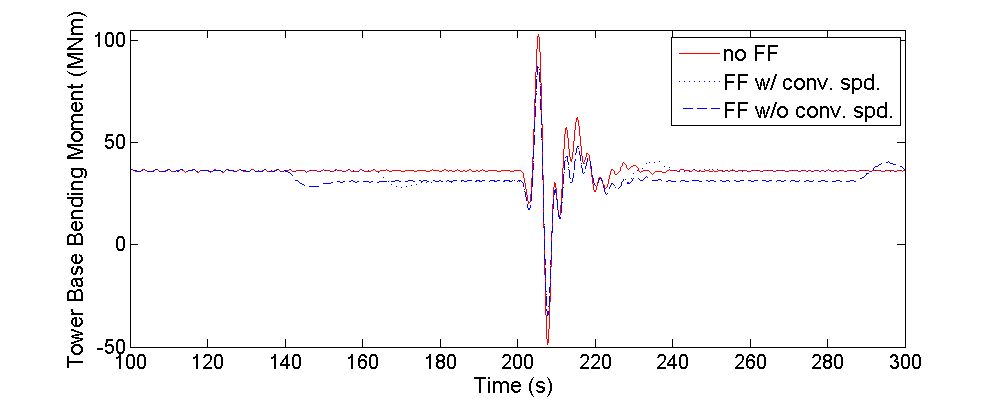
\includegraphics[width = \linewidth]{Figures/ch4Figures/fig4-24.png}
		
	\caption{Tower base fore-aft moment for turbine subjected to extreme operating gust.}
	\label{fig4-24}
\end{figure}

\begin{figure}[htbp]
	\centering
		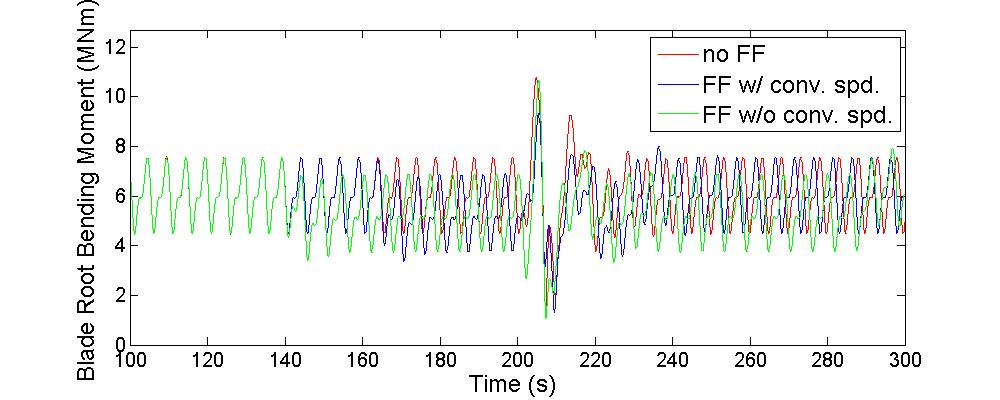
\includegraphics[width = \linewidth]{Figures/ch4Figures/fig4-25.png}
		
	\caption{Blade root bending moment for turbine subjected to extreme operating gust.}
	\label{fig4-25}
\end{figure}



These figures also illustrate that the system is robust to differences in the convection speed or errors in convection speed estimates. As discussed in section \ref{section3-2}, the simulation method used here assumes Taylor's frozen turbulence hypothesis, which implies that the true convection speed is equal to the mean wind speed. This assumption causes the EOG to reach the downwind turbine at exactly 200 seconds. However, if the EOG convects faster or slower than the mean wind speed the arrival time will shift. Similarly, if a convection velocity estimate is used to determine when to derate the downwind turbine then an error in the convection velocity estimate will cause that window of derated operation to shift. As we can see from Figures \ref{fig4-23} through \ref{fig4-25} small shifts will not affect the performance of the feed forward controller because the downwind turbine will still be in derated operation when the EOG arrives.

Figure \ref{fig4-25} shows power generation. As expected, derating the downwind turbine results in reduced power generation. When the derate timing is based on a convection velocity estimate it results in a loss of 11.5 KWh. If energy is sold at 10 cents per kWh that results in \$1.16 of lost revenue. When a convection velocity estimate is not used for derate timing the downwind turbine remains derated longer. This results in a loss of 26.48 kWh and lost revenue of approximately \$2.65. These simulations appear to show that turbines with feed forward selective derating control will generate less energy, however in real world operation this derating strategy may result in a significant increase in energy generation. It is important to note that these simulations do not model emergency rotor overspeed shutdowns. The turbine without feed forward control experiences a rotor overspeed of 18.76\%. If this caused a 10 minute emergency shutdown it would result in a loss of approximately 833 kWh and lost revenue of approximately \$83, significantly more than the lost revenue cased by briefly derating the turbine.

\begin{figure}[htbp]
	\centering
		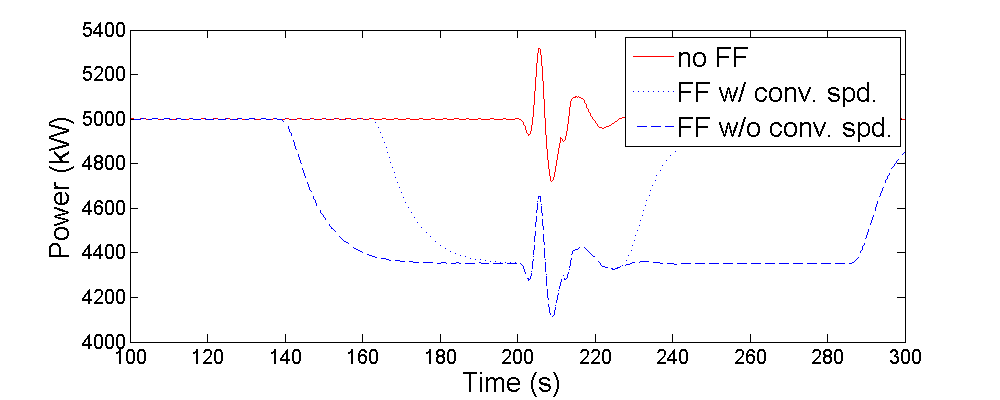
\includegraphics[width = \linewidth]{Figures/ch4Figures/fig4-26.png}
		
	\caption{Power generation for turbine subjected to extreme operating gust.}
	\label{fig4-26}
\end{figure}


\begin{table}[htbp]
\centering
\label{table4-3}
\begin{tabular}{c|cccccccccc}
\hline
\hline
                                                                &  & \multicolumn{2}{c}{\begin{tabular}[c]{@{}c@{}}Max Tower\\ Base Moment\end{tabular}} &  & \multicolumn{2}{c}{\begin{tabular}[c]{@{}c@{}}Max Blade\\ Root Moment\end{tabular}} &  & \begin{tabular}[c]{@{}c@{}}Max\\ Overspeed\end{tabular} &  &  \begin{tabular}[c]{@{}c@{}}Energy\\ Gen.\end{tabular}\\ 
                                                                     \cline{3-4}                                                                                    \cline{6-7}                                                                                       \cline{9-9}                                                           \cline{11-11} 
                                                                &  & (MNm)                                        & Reduction                                    &  & (MNm)                                        & Reduction                                    &  & (\%)                                                          &  &    (kWh)                         \\ 
\hline
\begin{tabular}[c]{@{}c@{}}No FF\\ Control\end{tabular}         &  & 102.7                                        & -                                            &  & 10.77                                        & -                                            &  & 18.76                                 						 &  &  831.8                                     \\
\\
\begin{tabular}[c]{@{}c@{}}FF w/ \\Conv. \\Speed\end{tabular} &  & 87.46                                        & 14.9\%                                       &  & 9.43                                        & 12.4\%                                        &  & 4.96                                                          &  &  820.2                                 \\
\\
\begin{tabular}[c]{@{}c@{}}FF w/o \\Conv. \\Speed\end{tabular}  &  & 87.34                                        & 15.0\%                                       &  & 10.66                                        & 1.0\%                                        &  & 4.96                                                          &  &  805.3                                 \\
\hline
\hline                             
\end{tabular}
\caption{Effect of FF Control on dynamic response to 16 m/s EOG.}
\end{table}





%-----------------------------------
%	SUBSECTION 4-6-2
%-----------------------------------
\subsection{Response to Turbulent Wind With Large Gust} \label{section4-6-2}

The Extreme Operating Gust test case provides insight into how selective derating can reduce loading and overspeeds. However, constant wind speeds like those before and after the EOG in the previous section, are rare in the real world. When a turbine experiences a large gust it is most likely part of a turbulent wind field. In this section we examine the effect of selective derating feed forward control on a two turbine system experiencing turbulent wind with a large gust. As discussed in Section \ref{section4-5}, the NREL 5-MW turbine is vulnerable to large gust induced overspeeds when operating in region 3 control, which occurs in wind speeds between 12 m/s and 25 m/s. As Section \ref{section4-3} illustrates, structural loading and overspeeds vary across that range of wind speeds. In an effort to capture these variations, turbulent wind speeds with 3 different mean wind speeds were simulated. Figures \ref{fig4-27} through \ref{fig4-31} illustrate the 16 m/s turbulent wind test case, while Tables \ref{table4-4} through \ref{table4-6} quantify and summarize performance metrics for all test cases. For the sake of space, the 12 m/s and 20 m/s turbulent wind test cases are not illustrated with figures. However, the behavior seen in the 12 m/s and 20 m/s test cases is similar to what is seen in the 16 m/s case.


Figure \ref{fig4-27} shows the wind speed for 200 seconds of the 16 m/s turbulent test case. As the figure shows, the turbines are subjected turbulent fluctuations in wind speed throughout the simulation with a large gust at 200 seconds. The turbulent fluctuations were generated by TurbSim and are statistically realistic, however these wind speeds are applied uniformly over the whole rotor. Due to the limitations of FAST and TurbSim it was not possible to simulate full field turbulence with a large gust, so the spatial variations in wind speed that would be observed across the rotor in a real turbulent wind field could not be captured in this simulation.

\begin{figure}[htbp]
	\centering
		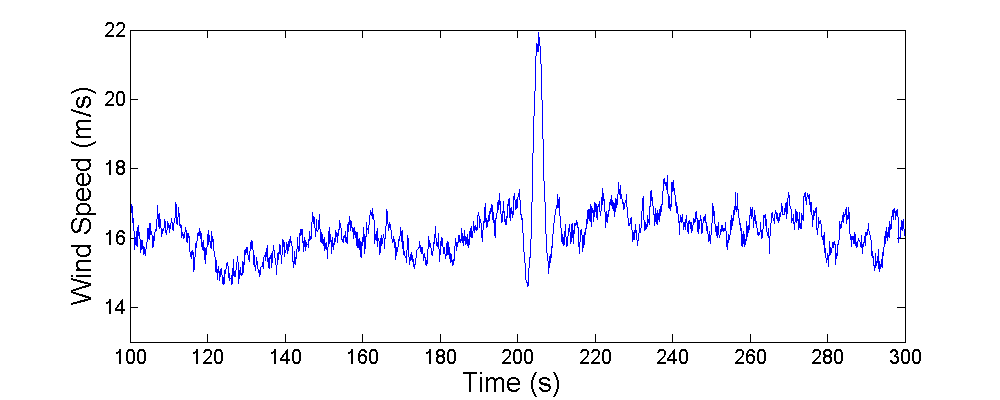
\includegraphics[width = \linewidth]{Figures/ch4Figures/fig4-27.png}
		
	\caption{Turbulent wind with 16 m/s mean wind speed and large gust.}
	\label{fig4-27}
\end{figure}

Figures \ref{fig4-28} through \ref{fig4-31} show how feed forward selective derating control affects the rotor speed, tower base fore-aft bending moment, blade root moment, and power generation of the downwind turbine for 16 m/s turbulent wind with a large gust. As in Section \ref{section4-6-1} two methods were used to time the derating of the downwind turbine.

Figure \ref{fig4-28} shows that the upwind turbine experiences many small overspeeds throughout the simulation and experiences a large overspeed of 17.77\% due to the large gust. This large overspeed could potentially cause an emergency overspeed shutdown of the upwind turbine. Selective derating feed forward control reduces the maximum overspeed experienced by the downwind turbine to approximately 5\%, which is in the normal range of operation for this turbine. In Figure \ref{fig4-29} we see that both the upwind and downwind turbines experience large tower base fore-aft bending moments due to the large gust, but the loads experienced by the downwind turbine are smaller. The feed forward controller has reduced the maximum tower base fore-aft bending moment by approximately 11\%. As in the previous section, we see that this system would be robust to changes in the arrival time of the gust. 

\begin{figure}[htbp]
	\centering
		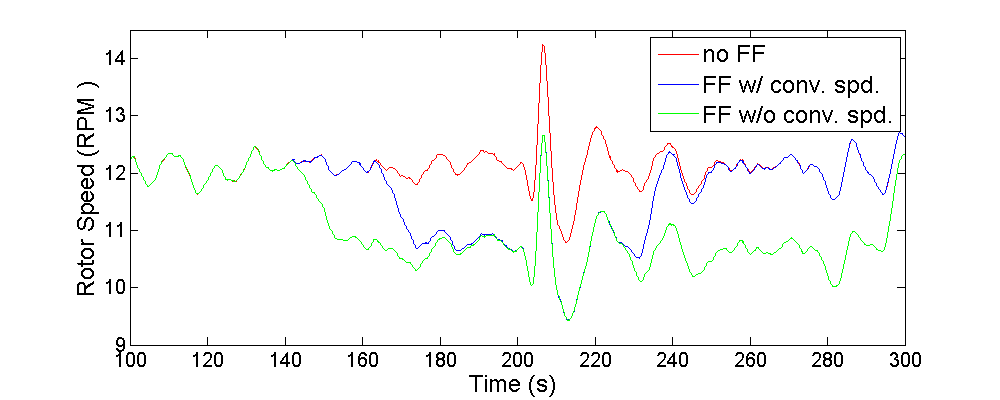
\includegraphics[width = \linewidth]{Figures/ch4Figures/fig4-28.png}
		
	\caption{Rotor speed for turbine subjected to turbulence w/ large gust.}
	\label{fig4-28}
\end{figure}

\begin{figure}[htbp]
	\centering
		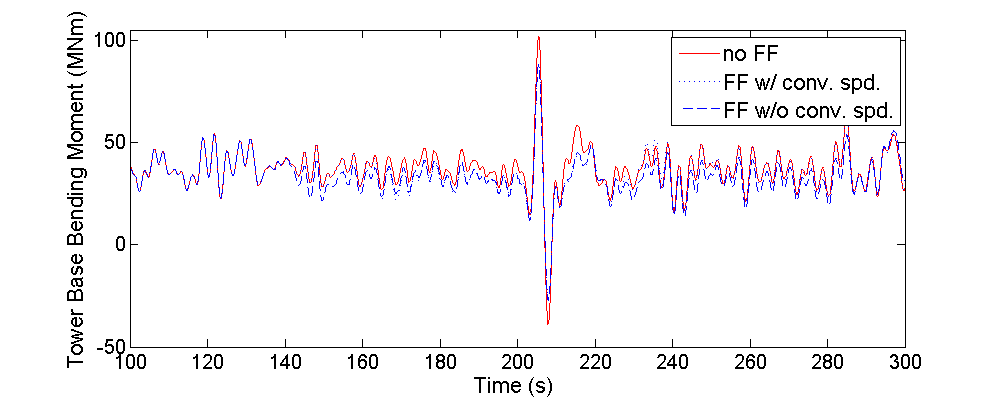
\includegraphics[width = \linewidth]{Figures/ch4Figures/fig4-29.png}
		
	\caption{Tower base fore-aft moment for turbine subjected to turbulence w/ large gust.}
	\label{fig4-29}
\end{figure}

Figure \ref{fig4-30} shows that derating the downwind turbine for the 16 m/s test case has resulted in a higher peak blade root moment (BRM). Though this result is initially surprising, it can be explained when the factors contributing to the peak load are examined more closely. We can see from Figure \ref{fig4-30} that BRM has a large cyclical component. These cyclic changes in BRM have a frequency of 12 RPM, which corresponds to the rotational speed of the rotor, and are caused primarily by gravitational loads on the turbine blade. Section \ref{section4-3} showed that derating reduces BRM, and we see from Figure \ref{fig4-30} that derating reduces BRM prior to the arrival of the gust. However, the effect of a large gust on BRM is determined by both how much BRM the gust causes as well as the timing of the gust and how the gust induced loads interacts with the cyclic gravitational loads. For the upwind turbine, without derating, the gust arrives at an opportune time. A downswing in the cyclic gravitational loading largely cancels out the gust induced BRM and the effect of the gust is almost unnoticeable. For the downwind turbine, the derating process has reduced the rotational speed of the rotor. As a result, the downwind turbine is at a different and less opportune point in it's rotation when the gust arrives. In real world applications the timing of a large gust would be random. Because derating reduces the BRM induced by the gust we would expect derating to reduce peak BRM more often than not. However, as this result illustrates, derating does not always result in reduced peak BRM loads.

\begin{figure}[htbp]
	\centering
		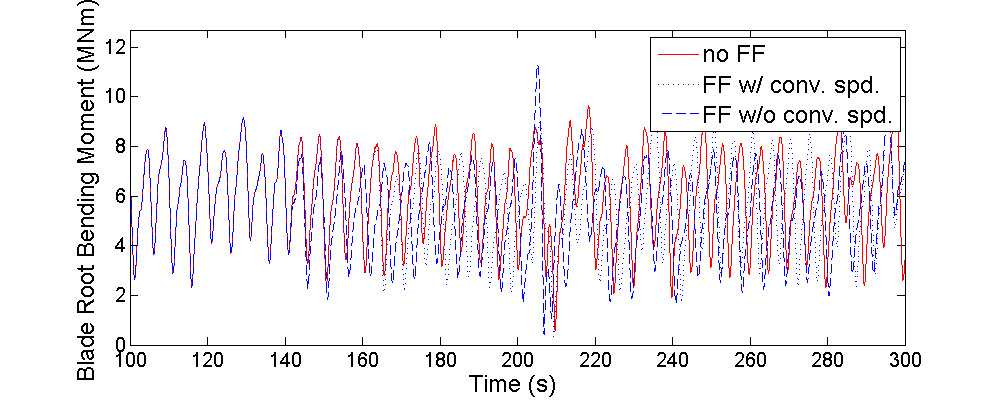
\includegraphics[width = \linewidth]{Figures/ch4Figures/fig4-30.png}
		
	\caption{Blade root bending moment for turbine subjected to turbulence w/ large gust.}
	\label{fig4-30}
\end{figure}

Figure \ref{fig4-31} shows power generation. As expected, derating results in reduced power generation. Derating based on a convection speed estimate results in 10.7 kWh of lost energy production. The more conservative strategy of derating without a convection speed estimate results in 24.9 kWh of lost energy production. However, as stated before, these derating strategies are intended to avoid emergency overspeed shut downs. An emergency overspeed shutdown would likely result in a much larger loss of energy.

\begin{figure}[htbp]
	\centering
		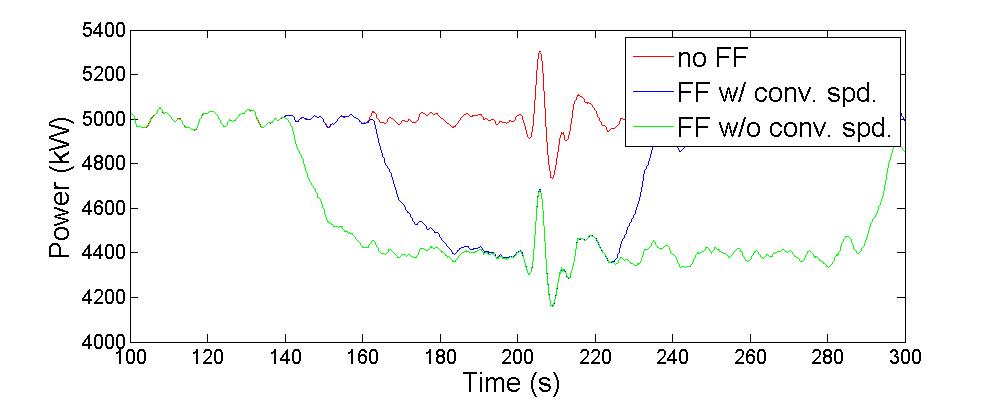
\includegraphics[width = \linewidth]{Figures/ch4Figures/fig4-31.png}
		
	\caption{Power generation for turbine subjected to turbulence w/ large gust.}
	\label{fig4-31}
\end{figure}

Tables \ref{table4-4} through \ref{table4-6} quantify and summarize performance metrics for all three test cases: 12 m/s, 16 m/s, and 20 m/s. In an attempt to capture the overall wear and tear on the tower base and blade root, Damage Equivalent Loads (DEL) are reported instead of peak loads. Though the DEL, overspeed, and energy generation values vary between the test cases, the trends are the same. Selective feed forward derating reduces maximum overspeeds from more than 15\%, which could cause an emergency overspeed shut down, to approximately 5\%. Tower root bending DELs are significantly reduced for all test cases. Blade root moment DELs are reduced in some test cases, but increased in others. Energy production is reduced by tens of kWh, which is equivalent to a few dollars of production.


\begin{table}[htbp]
\centering
\label{table4-4}
\begin{tabular}{c|cccccccccc}
\hline
\hline
                                                                &  & \multicolumn{2}{c}{\begin{tabular}[c]{@{}c@{}}Tower Base\\ DEL\end{tabular}} &  & \multicolumn{2}{c}{\begin{tabular}[c]{@{}c@{}}Blade Root\\ DEL\end{tabular}} &  & \begin{tabular}[c]{@{}c@{}}Max\\ Overspeed\end{tabular} &  &  \begin{tabular}[c]{@{}c@{}}Energy\\ Gen.\end{tabular}\\ 
                                                                     \cline{3-4}                                                                                    \cline{6-7}                                                                                       \cline{9-9}                                                           \cline{11-11} 
                                                                &  & (MNm)                                        & Reduction                                    &  & (MNm)                                        & Reduction                                    &  & (\%)                                                          &  &    (kWh)                         \\ 
\hline
\begin{tabular}[c]{@{}c@{}}No FF\\ Control\end{tabular}         &  & 78.8                                        & -                                            &  & 6.74                                        & -                                            &  & 15.79                                 						 &  &  812.1                                     \\
\\
\begin{tabular}[c]{@{}c@{}}FF w/ \\Conv. \\Speed\end{tabular} &  & 69.2                                        & 12.2 \%                                       &  & 5.87                                        & 12.9\%                                        &  & 4.46                                                          &  &  800.9                                 \\
\\
\begin{tabular}[c]{@{}c@{}}FF w/o \\Conv. \\Speed\end{tabular}  &  & 67.5                                        & 14.3\%                                       &  & 5.16                                        & 23.2\%                                        &  & 4.46                                                          &  &  790.98                                 \\
\hline
\hline                             
\end{tabular}
\caption{Effect of FF Control on damage equivalent loads for a large gust in turbulent wind with 12 m/s mean wind speed.}
\end{table}


\begin{table}[htbp]
\centering
\label{table4-5}
\begin{tabular}{c|cccccccccc}
\hline
\hline
                                                                &  & \multicolumn{2}{c}{\begin{tabular}[c]{@{}c@{}}Tower Base\\ DEL\end{tabular}} &  & \multicolumn{2}{c}{\begin{tabular}[c]{@{}c@{}}Blade Root\\ DEL\end{tabular}} &  & \begin{tabular}[c]{@{}c@{}}Max\\ Overspeed\end{tabular} &  &  \begin{tabular}[c]{@{}c@{}}Energy\\ Gen.\end{tabular}\\ 
                                                                     \cline{3-4}                                                                                    \cline{6-7}                                                                                       \cline{9-9}                                                           \cline{11-11} 
                                                                &  & (MNm)                                        & Reduction                                    &  & (MNm)                                        & Reduction                                    &  & (\%)                                                          &  &    (kWh)                         \\ 
\hline
\begin{tabular}[c]{@{}c@{}}No FF\\ Control\end{tabular}         &  & 75.1                                        & -                                            &  & 5.08                                        & -                                            &  & 17.77                                 						 &  &  831.8                                     \\
\\
\begin{tabular}[c]{@{}c@{}}FF w/ \\Conv. \\Speed\end{tabular} &  & 67.2                                        & 10.5 \%                                       &  & 5.14                                        & -1.2\%                                        &  & 5.04                                                        &  &  821.1                                 \\
\\
\begin{tabular}[c]{@{}c@{}}FF w/o \\Conv. \\Speed\end{tabular}  &  & 66.3                                        & 11.7\%                                       &  & 5.44                                        & -7.1\%                                        &  & 4.88                                                          &  &  806.9                                 \\
\hline
\hline                             
\end{tabular}
\caption{Effect of FF Control on damage equivalent loads for a large gust in turbulent wind with 16 m/s mean wind speed.}
\end{table}

\begin{table}[htbp]
\centering
\label{table4-6}
\begin{tabular}{c|cccccccccc}
\hline
\hline
                                                                &  & \multicolumn{2}{c}{\begin{tabular}[c]{@{}c@{}}Tower Base\\ DEL\end{tabular}} &  & \multicolumn{2}{c}{\begin{tabular}[c]{@{}c@{}}Blade Root\\ DEL\end{tabular}} &  & \begin{tabular}[c]{@{}c@{}}Max\\ Overspeed\end{tabular} &  &  \begin{tabular}[c]{@{}c@{}}Energy\\ Gen.\end{tabular}\\ 
                                                                     \cline{3-4}                                                                                    \cline{6-7}                                                                                       \cline{9-9}                                                           \cline{11-11} 
                                                                &  & (MNm)                                        & Reduction                                    &  & (MNm)                                        & Reduction                                    &  & (\%)                                                          &  &    (kWh)                         \\ 
\hline
\begin{tabular}[c]{@{}c@{}}No FF\\ Control\end{tabular}         &  & 91.1                                        & -                                            &  & 5.08                                        & -                                            &  & 22.89                                 						 &  &  831.8                                     \\
\\
\begin{tabular}[c]{@{}c@{}}FF w/ \\Conv. \\Speed\end{tabular} &  & 77.2                                        & 15.3 \%                                       &  & 5.06                                        & 0.3\%                                        &  & 5.04                                                          &  &  818.8                                 \\
\\
\begin{tabular}[c]{@{}c@{}}FF w/o \\Conv. \\Speed\end{tabular}  &  & 76.6                                        & 15.9\%                                       &  & 5.20                                        & -2.4\%                                        &  & 5.12                                                          &  &  798.5                                 \\
\hline
\hline                             
\end{tabular}
\caption{Effect of FF Control on damage equivalent loads for a large gust in turbulent wind with 20 m/s mean wind speed.}
\end{table}






%----------------------------------------------------------------------------------------
%	SECTION 4-7
%----------------------------------------------------------------------------------------

\section{Conclusions.} \label{section4-8}

This chapter has investigated the benefits and feasibility of derating a downwind turbine based on a feed forward signal from an upwind turbine. A survey of available turbine derating literature was carried out. Three turbine derating strategies from literature were then investigated. It was found that derating a turbine by reducing the rated rotor speed yielded the largest reductions in structural loads and rotor overspeeds. The effect of turbine derating on dynamic turbine response was then investigated by simulating derated NREL 5-MW turbines subjected to extreme operating gusts (EOGs). It was found that rotor speed, power, blade root bending moments, and tower fore-aft bending moments were all significantly reduced by derating and that the reduction were roughly proportional to the amount of derating. The transition into and out of derated mode was also investigated. It was found that abruptly changing the rating of an NREL 5-MW turbine excited undesirable transient behavior in the turbine. However, the undesirable behavior could be avoided by using a low pass filter. A feed forward selective derating scheme based on these findings was developed. The scheme uses two possible methods to determine when to derate the downwind turbine. The first relies on a wind convection velocity estimate from the upwind turbine. The second, more conservative, method uses the range of wind speeds in which rotor overspeeds are likely to occur. 

Once the feed forward selective derating strategy was designed, the performance of that system was tested in a series of FAST simulations. The FAST simulations modeled a two turbine system in several wind conditions, including both  IEC Extreme Operating Gusts and turbulent wind with large gusts. The simulation results were promising. The downwind turbine experienced significant reductions in tower fore-aft moments in all simulation cases, as well as reductions in blade root bending moments in some cases. More importantly, the downwind turbine did not experience any rotor overspeeds large enough to trigger an emergency shut down. The downwind turbine experienced reductions in energy generation, however those reductions were much smaller than the reductions in energy generation that would be caused by an emergency overspeed shut down.

Though the simulations carried out in this chapter show promising system performance, more investigation is needed. A real wold implementation of this system would encounter several phenomena that were not captured in these simulation. Due to the limitations of the simulation tools, neither full field turbulence nor the evolution of the wind field over time could be simulated. In addition simulating the system with a different simulation tool could potentially lend validity to the results shown in this chapter. In the following chapters a more sophisticated, though more computationally intensive, wind farm simulation tool will be investigated and used to study the feed forward selective derating scheme developed in this chapter.
